\lettrine{C}{loud} computing has reshaped how companies build software, shifting the focus to \textbf{scalable solutions} that leverage \textbf{elastic infrastructure}. 
Applications are increasingly \textbf{containerized} and managed with platforms such as \textbf{Kubernetes}, while \textbf{serverless computing} has also gained traction.  

\vspace{0.5em} Being inherently \textbf{distributed}, \textbf{cloud-native systems} face the challenges outlined by the \textbf{CAP theorem}: architects must balance \textbf{Partition Tolerance}, \textbf{Consistency}, and \textbf{Availability}. 
This has led to designs that relax \textbf{strong consistency} in favor of \textbf{availability} through \textbf{Eventual Consistency}.  

\begin{boxF}
    The \textbf{CAP theorem} \cite{c1} states that, in the presence of a \textbf{network partition}, a system must trade off between \textbf{Consistency} and \textbf{Availability}. 
    \textbf{Eventual Consistency} aligns with \textbf{PA (Partition Tolerance and Availability)}, allowing a system to remain responsive during partitions while deferring full consistency until recovery. 
\end{boxF}

\begin{figure}[h]
    \centering
    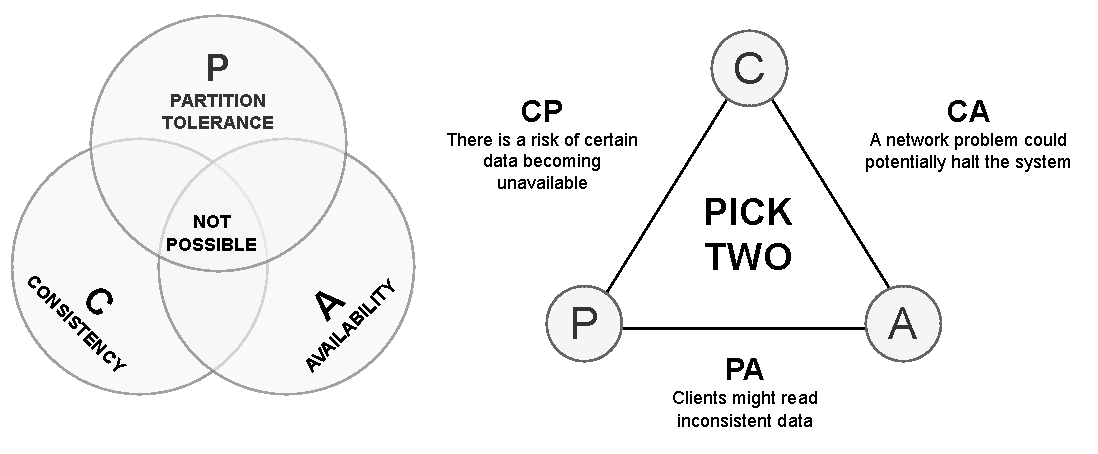
\includegraphics[width=\linewidth]{iezt/cap-theorem.pdf}
    \caption{CAP Theorem}
    \label{fig:cap-theorem}
\end{figure}

Another major trend is the adoption of \textbf{asynchronous patterns} and \textbf{event-streaming frameworks} such as \textbf{Apache Kafka}, which handle continuous flows of events without a clear beginning or end.  
In this setting, \textbf{orchestration} has proven complex and difficult to scale, whereas \textbf{choreography-based systems} often provide better scalability.  

Figure \ref{fig:cloud-architecture} shows a typical \textbf{cloud architecture}: clients authenticate with a centralized \textbf{Identity Provider}, which issues a \textbf{token} subsequently used to access server resources. 
Two widely adopted protocols here are \textbf{OpenID} \cite{c4} for authentication and \textbf{OAuth} \cite{c5} for authorization.  

\begin{figure*}[htbp]
    \centering
    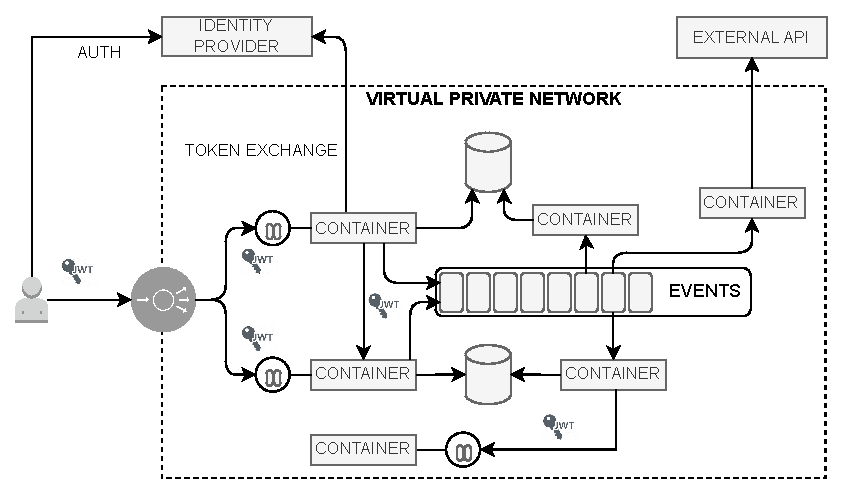
\includegraphics[width=0.7\textwidth]{iezt/cloud-architecture.pdf}
    \caption{Cloud Architecture}
    \label{fig:cloud-architecture}
\end{figure*}

\vspace{0.5em} Within these protocols, \textbf{JSON Web Tokens (JWT)} \cite{c6} have become central. 
Compact and digitally signed, they ensure \textbf{message integrity} and enable \textbf{secure communication} between client and server.  

\vspace{0.5em} \textbf{Access control} remains a critical concern. Models such as \textbf{Role-Based Access Control (RBAC)} and \textbf{Attribute-Based Access Control (ABAC)} have paved the way for \textbf{Policy-Based Access Control (PBAC)} \cite{c7}.  

\vspace{0.5em} A further challenge arises in \textbf{transport-layer communication}, for example with \textbf{Kafka} and \textbf{stream-processing systems}, where it is not always feasible to propagate a token.

\begin{figure}[htbp]
    \centering
    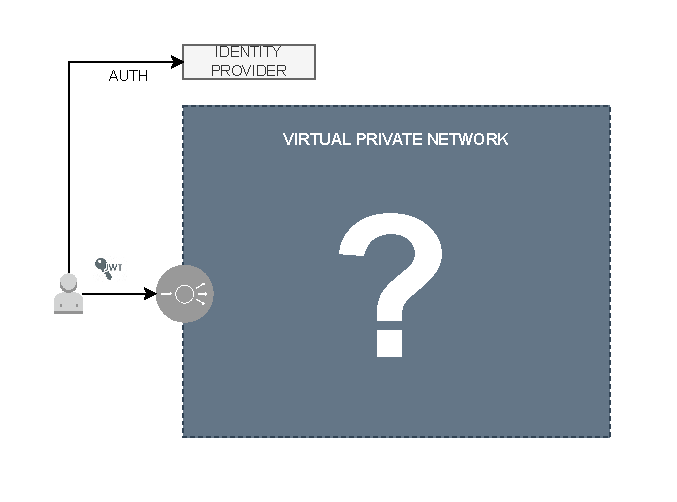
\includegraphics[width=0.5\textwidth]{iezt/current-model.pdf}
    \caption{Building inside a Perimeter}
    \label{fig:current-model}
\end{figure}

\vspace{0.5em} This exposes a key limitation of the \textbf{current model}: it works at the \textbf{perimeter}, where \textbf{tokens} are validated at delivery, but what happens \textbf{inside the enterprise} afterward is not standardized. 
\textbf{Authorization} is essentially assumed to remain valid once accepted at the boundary, and the system continues to treat it as true for the rest of the time.  
While this trade-off was once acceptable, it cannot be sustained in environments that must support \textbf{AI agents}.  

Moreover, modern \textbf{distributed systems} increasingly operate \emph{without clear perimeters}. 
In \textbf{cloud-native}, \textbf{multi-tenant}, and \textbf{hybrid environments}, workloads, services, and agents continuously interact across organizational and network boundaries. 
In such scenarios, the very assumption of a \textbf{fixed perimeter} for validation no longer holds, making \textbf{token-based authorization} even more fragile.  

It follows that the \textbf{current model} is not suitable for \textbf{AI agents}, which require \textbf{dynamic}, \textbf{context-aware}, and \textbf{continuously validated authorization}. 
The goal is not to replace existing protocols but to complement them, addressing the \textbf{gaps} they have historically overlooked.
